% Standard RL loop for LLMs — agent <-> environment.
% Root of the "RL feedback loop" family (see rlhf_loop, rlvr_loop, tooluse_rl).
\documentclass{article}
\usepackage[margin=0.4cm, paperwidth=15cm, paperheight=10cm]{geometry}
\usepackage{tikz}
\usepackage{lmodern}
\renewcommand{\familydefault}{\sfdefault}
\usetikzlibrary{positioning, arrows.meta, calc}
\pagestyle{empty}

\definecolor{agentorange}{RGB}{245,166,35}
\definecolor{envgreen}{RGB}{39,174,96}
\definecolor{arrownavy}{RGB}{46,49,146}

\begin{document}
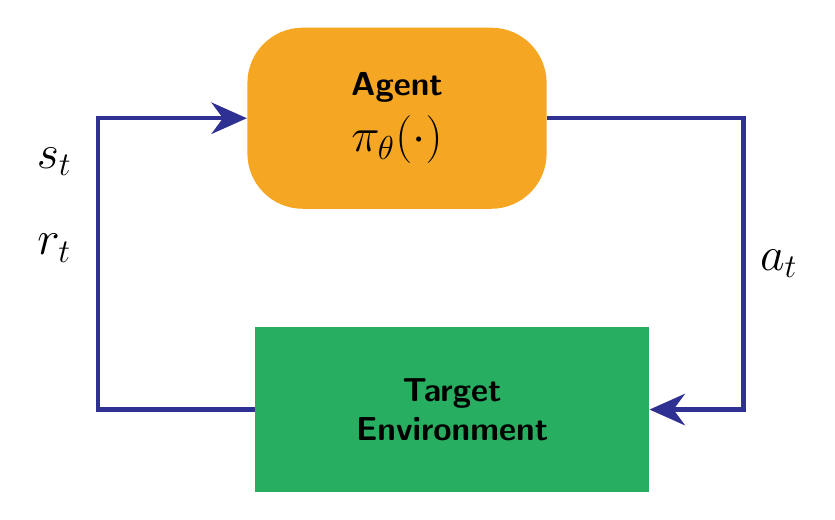
\begin{tikzpicture}[
    agent/.style={
        rectangle, rounded corners=20pt, fill=agentorange,
        minimum width=3.8cm, minimum height=2.3cm,
        align=center, font=\large\bfseries, text=black
    },
    env/.style={
        rectangle, fill=envgreen,
        minimum width=5.0cm, minimum height=2.1cm,
        align=center, font=\large\bfseries, text=black
    },
    loop/.style={
        -{Stealth[length=4.5mm, width=4mm]},
        line width=1.5pt, color=arrownavy
    },
    edgelbl/.style={font=\LARGE}
]

% --- nodes ---
\node[agent] (agent) at (0,0) {Agent\\[4pt]{\LARGE$\pi_\theta(\cdot)$}};
\node[env]   (env)   at (0.7,-3.7) {Target\\Environment};

% --- action: agent -> environment (right side, down) ---
\draw[loop] (agent.east) -- (4.4,0) -- (4.4,-3.7) -- (env.east);
\node[edgelbl] at (4.85,-1.85) {$a_t$};

% --- state + reward: environment -> agent (left side, up) ---
\draw[loop] (env.west) -- (-3.8,-3.7) -- (-3.8,0) -- (agent.west);
\node[edgelbl] at (-4.35,-0.55) {$s_t$};
\node[edgelbl] at (-4.35,-1.65) {$r_t$};

\end{tikzpicture}
\end{document}
